%%%% ijcai11.tex

\typeout{IJCAI-11 Instructions for Authors}

% These are the instructions for authors for IJCAI-11.
% They are the same as the ones for IJCAI-07 with superficical wording
%   changes only.

\documentclass{article}
% The file ijcai11.sty is the style file for IJCAI-11 (same as ijcai07.sty).
\usepackage{ijcai11}

% Use the postscript times font!
\usepackage{times}

\usepackage[utf8]{inputenc}
\usepackage[catalan]{babel}

\usepackage{graphicx}

% the following package is optional:
%\usepackage{latexsym} 

% Following comment is from ijcai97-submit.tex:
% The preparation of these files was supported by Schlumberger Palo Alto
% Research, AT\&T Bell Laboratories, and Morgan Kaufmann Publishers.
% Shirley Jowell, of Morgan Kaufmann Publishers, and Peter F.
% Patel-Schneider, of AT\&T Bell Laboratories collaborated on their
% preparation.

% These instructions can be modified and used in other conferences as long
% as credit to the authors and supporting agencies is retained, this notice
% is not changed, and further modification or reuse is not restricted.
% Neither Shirley Jowell nor Peter F. Patel-Schneider can be listed as
% contacts for providing assistance without their prior permission.

% To use for other conferences, change references to files and the
% conference appropriate and use other authors, contacts, publishers, and
% organizations.
% Also change the deadline and address for returning papers and the length and
% page charge instructions.
% Put where the files are available in the appropriate places.

\title{Implementació de la teoria de resta de\\formes desenvolupada en el grup C4R2}
\author{Ivan Barrachina Bellmunt i Josep López Centelles\\
II-80 Intel·ligència Artificial avançada\\
Universitat Jaume I Castelló\\
Avda. Vicent Sos Baynat s/n, 12071 Espanya \\
al106647@uji.es, al106650@uji.es}

\begin{document}

\maketitle

\begin{abstract}
Aquest article explica el treball realitzat per a implementar la teoria de resta de formes definida pel grup C4R2 [Mus09].
Com a objectiu final s'ha obtingut una interfície gràfica que ens permet elegir dos figures, de les quals es calcula la resta, i es mostra tant el resultat com la seua descripció qualitativa.
\end{abstract}

\section{Introducció}
El treball que es planteja a continuació tracta de presentar la teoria de la resta de formes i la integració d'aquesta en una interfície gràfica.
Existeixen algunes limitacions que no permeten fer qualsevol resta de formes però s'ha intentat que aquesta versió del software accepte la majoria d'elles.
\\
\\
La intel·ligència artificial és considerada una rama de la computació i relaciona un fenomen natural amb una analogia artificial a través de programes de computador.
De manera més específica la intel·ligència artificial és la disciplina que s'encarrega de construir processos que al ser executats sobre una arquitectura física produeixen accions o resultats que maximitzen una mesura de rendiment determinada, basant-se en la seqüència de entrades percebudes i el coneixement emmagatzemat en dita arquitectura.
\\
\\
Aquest projecte es centra en la interpretació de les característiques qualitatives per a definir la nova figura.
L'analisis de característiques qualitatives és una de les facultats que té la ment humana i s'utilitza a diari.
Implementant aquest procés es dote al nostre software d'una intel·ligència artificial clara, ja que es simula una forma de pensar molt humana.
\\
\\
\subsection{Aquest treball dintre de la intel·ligència artificial}
El treball que a desenvolupar tracta sobre l'obtenció d'imatges, anàlisis de les seves característiques i finalment la realització d'una operació en la que s'utilitzen dos figures per obtindre el resultat de la seva resta.
Açò pot ser utilitzat posteriorment per a definir mosaics d'una forma intel·ligent i amb la seguretat d'evitar errors.
La primera part del projecte que consta de l'obtenció dels vèrtex d'una figura correspon al camp de la visió, mentre que l'anàlisi i els seus resultats pertanyen al camp del raonament qualitatiu, dins de la intel·ligència artificial.
\\
\section{Descripció qualitativa de les figures}
Com s'ha dit anteriorment, en aquest treball s'utilitzarà la descripció qualitativa de figures, obtinguda mitjançant l'executable desenvolupat en [Mus07].
La descripció qualitativa consisteix en l'assignació de valors de les principals característiques de cada vèrtex de la figura dins de rangs definits qualitativament.
En aquests rangs no hi ha valors enterns sino conceptes que determinen en quin rang es trova cadascuna dels valors reals.
Per exemple, un angle no es determina mitjançant el nombre de graus que conté sino que es descriurà definint el seu rang: molt agut, agut, recte, obert, molt obert.
\\
\\
Les característiques que determinen cada vèrtex són el tipus d'angle, la seua convexitat i la llargària de les seues arestes respecte les seues veïnes.
Per a poder exlicar com es realitzen els cálculs de la descripció qualitativa s'usaran els tres vèrtexs participants en cada càlcul.
S'anomenaran aquest punts com i(anterior), j(vèrtex que s'està calculant) i k(següent) per a facilitar l'explicació dels càlculs.
\\
\subsection{Tipus d'angle}
Per classificar l'angle del vèrtex j, es dibuixarà un cercle amb diàmetre i k, que és la línia d'unió entre els vèrtexs i (anterior) i k (següent).
Si el vèrtex que s'estudia es troba a l'interior del cercle, s'anomenarà obtús (obtuse), si es troba en l'exterior s’anomenarà agut (acute) i si coincideix en la circumferència serà recte (right).
\\
\\
A més, si els angles són molt aguts (0-40 graus) o molt obtusos (140-180 graus) es defineixen com very obtuse o very acute.
Es pot observar en la Figura~\ref{fig:angles} com es defineix alguns tipus d'angles.
\\

\begin{figure}[h]
\centering
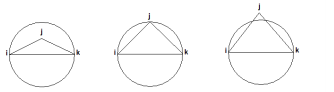
\includegraphics[width=260pt]{images/angles.png}
\caption {Exemples de l'estudi de la classificació de tres angles, un obtús, un recte i un tercer agut.}
\label {fig:angles}
\end{figure}

\subsection{Convexitat}
Per calcular el tipus de convexitat de l’angle del vèrtex j, es realitza una línia del vèrtex anterior al posterior.
Si aquest vèrtex j es troba a l'esquerra d'aquesta línia, es diu que l'angle és convex i si es troba a la dreta, còncau.
En la Figura~\ref{fig:convex} s'observen els dos posibles exemples de les diferents convexitats.

\begin{figure}[h]
\centering
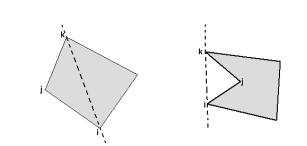
\includegraphics[width=260pt]{images/convex.jpeg}
\caption {Exemple de la convexitat de dos angles, un primer convex i un còncau.}
\label {fig:convex}
\end{figure}

\subsection{Llargària de les arestes}
Per calcular la llargària de les arestes del vèrtex  j, es comparara la distància euclídea de les línies i-j i j-k.
\\
\\
D(j-k)=)=((Xk-Xj)2+(Yk-Ykj)2)1/2
\\
\\
D(i-j)=)=((Xj-Xi)2+(Yj-Yki)2)1/2
\\
\\
Comparant aquestes dos dades obtenim el valor de la llargària de les arestes:
\begin{itemize}
\item Si D(j-k) = [0, 0,4]   D(i-k) $\rightarrow$  Molt menor (much-shorter)
\item Si D(j-k) = [0.4, 0.6] D(i-k) $\rightarrow$  Mitad (half-lenght)
\item Si D(j-k) = [0.6, 0.9] D(i-k) $\rightarrow$  Un poc menor (a-bit-shorter)
\item Si D(j-k) = [0.9, 1.1] D(i-k) $\rightarrow$  Igual (similar-lenght)
\item Si D(j-k) = [1.1, 1.9] D(i-k) $\rightarrow$  Un poc major (a-bit-longer)
\item Si D(j-k) = [1.9, 2.1] D(i-k) $\rightarrow$  Doble (double-lenght)
\item Si D(j-k) = [2.1, n]   D(i-k) $\rightarrow$  Molt major (much-longer)
\end{itemize}

\subsection{Connexió}
És el tipus d'aresta connectada i pot ser: connexió entre dos linees rectes (\emph{line-line}), una linea recta i una curva (\emph{line-curve}), dos linees curves (\emph{curve-curve}), una linea curva i una recta (\emph{curve-line}) o punto de curvatura (\emph{curvature-point}).
En el nostre cas al restar figures poligonals sempre serà \emph{line-line} ja que no s'ha tractat el problema de restar figures amb arestes que no siguen rectes.
\\
\\
\subsection{Descripció completa de la figura}
Ja explicades totes les característiques de cada vèrtex, sols es necessita definir un estandard per a mostrar tota la informació.
Iniciant desde el primer vèrtex (el que estiga més amunt i a l'esquerra) es va mostrant tota la informació de tots els vèrtexs com es pot veure en aquest exemple:
  
\begin{center}
\emph{[Con1,Cur1,Lon1,Conv1]...[ConN,CurN,LonN,ConvN]}
\end{center}

Aquest exemple respon a la descripció de vèrtex explicada en la teoria de [Zoe12], segons la qual els vèrtex d'una figura es descriuen com una tupla $<$ Con; Cur; Lon; Conv $>$ on:

\begin{itemize}
\item \emph{Con} és el tipus d'aresta conectada.
\item \emph{Cur} és la curvatura, l'angle del vèrtex.
\item \emph{Lon} és la longitud comparada de l'aresta anterior respecte a la següent.
\item \emph{Conv} és la convexitat del vèrtex.
\end{itemize}

Els valors de cadascuna de les anteriors característiques s'han definit anteriorment de forma que la descripció de la Figura~\ref{fig:exemple} sería la que es veu a continuació.
\\
\\
\emph{[line-line, right, a-bit-longer, convex], [line-line, right, a-bit-shorter, convex], [line-line, right, a-bit-longer, convex], [line-line, right, a-bit-shorter, convex]}

\begin{figure}[h]
\centering
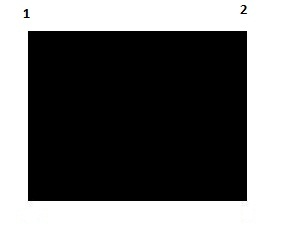
\includegraphics[width=260pt]{images/quad_gran.jpg}
\caption {Exemple de figura per a mostrar la seua descripció qualitativa.}
\label {fig:exemple}
\end{figure}

\subsection{Limitacions de les figures}
Quan es realitza una operació de diferència, existeix un minuend al que se li resta un substrahend per obtindre un resultat, la diferència. En el cas de restar figures, existeixe una sèrie de restriccions que aquetestes deuen cumplir per a que els càlculs funcionen correctament.
La diferència es realitzarà sempre per el primer vèrtex de la descripció de la figura minuend. Açò vol dir, per el vèrtex amb menor y i menor x (les x del plà van de esquerra a dreta i les y de amunt a aball).
\\
\\
El minuend sempre deu ser major que el substrahend, en el cas de les figures, per a comprovar que aquesta restricció es cumpleix, es deuen comprovar que ningun dels punts característics del substrahend es surt de la frontera del minuend.
Si el minuend té diferents amplaries es considerà que la resta no es pot realitzar si el substrahend supera l'amplaria de la part superior del minuend. 
Com a cas base si les dos figures són iguales, es a dir, són la mateixa figura el resultat serà una figura sense vèrtexs i un mensaje d'error.
\\
\\
Les figures no poden tenir segments que no siguen rectes ja que la existencia de linees curves dificultaria molt els cálculs.
Ademés si la resta produeix més d'una figura en el nostre programa només es tindrà en compte una d'aquestes figures ignorant a les altres.
S'intenta sempre elegir la figura més gran de les posibles i es considera que la resta es pot omplir amb masilla.
\\
\\
Les figures han de estar orientades de forma que el seu primer punt (de situat més amunt i més a l'esquerra) es puga colocar en l'origen de coordenades (0,0).
D'aquesta forma sempre es resta per la part de dalt i el màxim a l'esquerra posible.
Estrategia que dòna ordre a les restes consecutives de figures sobre una figura inicial.
\\

\section{Diferència de formes}
Una vegada explicada la teoria de descripció qualitativa de formes a partir de l'estudi dels seus vèrtexs, sols ens queda passar a presentar la teoria sobre com calcular la descripció qualitativa d'una nova figura, creada a partir de la  diferència de dues figures simples de les que ja es coneixen la seva descripció.
Cadascuna de les característiques dels vèrtexs s'han de calcular de forma independent per a cada vèrtex.
En les següents seccions s'explica com s'obté el valor de cadascun d'aquests.

\subsection{Càlcul del tipus d'angle dels nous vèrtexs}
Els angles dels nous vèrtex es calcularan depenent de si aquestos fan frontera o no amb el minuend.
S’utilitzarà la Taula~\ref{fig:taula1} per calcular l’angle de la nova figura en els dos següents casos:

\begin{itemize}
\item En el cas que hi fagen frontera, el nou angle serà el suplementari al del subtrahend.
      Açò vol dir que si el angle del subtrahend era \emph{very-acute}, el nou serà \emph{very-obtuse};
      si era \emph{acute}, el nou serà \emph{obtuse};
      si era \emph{right}, el nou serà \emph{right};
      si era \emph{obtuse} el nou serà \emph{acute};
      i si era \emph{very-obtuse} el no serà \emph{very-acute}.

\item Els vèrtex dels subtrahend que no hi facen frontera amb el minuend es convertiran en vèrtex còncaus de la nova figura, amb el mateix tipus d’angle.
\end{itemize}

\begin{figure}[h]
\centering
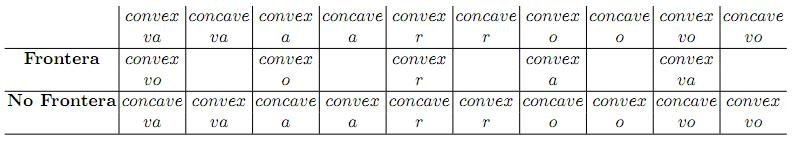
\includegraphics[width=260pt]{images/taula1.jpeg}
\caption {Angles que forma el substrahend en la nova figura, depenent del àngle original.}
\label {fig:taula1}
\end{figure}

Es possible que al realitzar la diferència algun vèrtex del substrahend diferent al que estem restant ocupe la mateixa posició que un altre vèrtex del minuend.
En aquest cas, sols serà possible ficar la peça si l’angle del vèrtex del substrahen és menor o igual al del minuend.
En cas que siguen iguals o complementaris (la resta done 180, açò sols es pot donar si un angle és cóncau i l’altre convex), el vèrtex desapareix.
En cas que siga menor, en la Taula~\ref{fig:taula2} es poden comprobar l’angle resultant.

\begin{figure}[h]
\centering
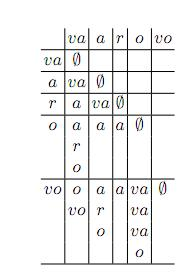
\includegraphics[width=100pt]{images/taula2.jpeg}
\caption {En la taula es mostra l’angle resultant de restar-li a un angle tipus fila un angle tipus columna.}
\label {fig:taula2}
\end{figure}


Quan són del mateix tipus es considera que s’anula ( ja que encara que no siguen idèntics es pot ficar massilla per fer el trencadís).
Algunes indeterminacións també es poden eliminar considerant que es posa massilla.
Per a simplificar en els casos en els que hi ha diverses solucions posibles es considera la més provable d'elles.
D'esta forma la taula quedarà com es mostra en la Taula~\ref{fig:taula3}.

\begin{figure}[h]
\centering
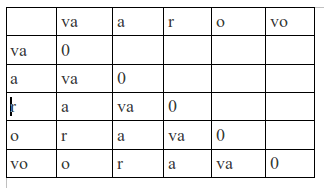
\includegraphics[width=160pt]{images/taula3.png}
\caption {Càlculs simplificats de la resta d'angles.}
\label {fig:taula3}
\end{figure}


\subsection{Càlcul del tipus de convexitat dels nous vèrtexs}
El cálcul de la convexitat està molt relacionat en el càlcul del tipus d'angle de la nova figura.
Es pot observar com es modifiquen els valors de la convexitat en la Taula~\ref{fig:taula1}.
Depenent de si el vertex pertany a la frontera del minuend o no es modificarà el seu valor o es mantindrà l'antic.
\\
\\
\subsection{Càlcul de la llargària de les arestes de la nova figura}
En cas que desaparega un vèrtex per restar dos angles complementaris, haurà que calcular la longitud de la nova aresta amb l’angle anterior i el següent.
La longitud de les arestes afectades en la resta deurà calcularse qualitativament, setant-li a la longitud de les arestes del minuend, la longitud de les del sustrahend.
Una volta calculades les noves longituts, es calcula la longitud comparada per añadir-la a la nova descripció.
\\
\\
\subsection{Càlcul del tipus connexió dels nous vèrtexs}
A l'existir la limitació de que totes les figures han de ser polígons amb tots els seus costats rectes aquest càlcul serà molt simple.
En tots els vèrtexs el valor del tipus de connexió serà \emph{line-line}. 
\\
\\
\section{Formació de la nova figura}
Per a realitzar la resta de dos figures un dels passos més difícils consisteix en la definició dels vertexs de la nova figura.
S'han de considerar tots els vèrtexs com a posibles integrants de la nova figura.
Però mitjançant diverses comprovacions s'arriba a la llista final del vèrtexs de la figura final.
\\
\\
Abans de treballar amb els vertexs s'han d'igualar les posicions de les dos figures.
Considetant com a punt principal el situat més amunt i a l'esquerra, es modifiquen tots els valors de tots els punts de forma que aquest punt estigue en l'eix de coordenades.
Ocorre un problema si la figura té una forma que produeix que alguns dels seus punts es situen a la zona negativa dels eixos x o y.
Per solucionar açò disposem d'un altra funció que mou la figura per a que torne a una posició correcta.
\\
\\
El procés consisteix en descartar els punts coincidents tant per davant com per detràs.
Posteriorment es recorren els vèrtexs restants de forma ordenada.
Aquest procés s'explica en molt més de detall en els següents apartats.
\\
\\
\subsection{Descartar punts}
Tenint en compte que el primer vèrtex en la llista de punts de cada figura s'encontrarà en la posició (0,0) s'inicia el recorregut dels següents punts.
Aquest primer vèrtex es descarta directament per a formar part de la nova figura.
Si el segon punt de les dos figures també coincideixen significa que tampoc formaran part de la nova figura.
Es segueix recorrent els punt fins trovar un parell que no siguen iguals.
Aquests seran els dos primers punts de la nova figura.
\\
\\
Tots els punts que han coincidit en les dos figures es marquen com a visitats i no es consideraran per a formar la nova figura. 
Aquest procés es repeteix recorrent els vèrtexs des dels últims, per a descartar també els que coincideixen  
\\
\\
\subsection{Primer punt del substrahend}
Per a iniciar la formació de la figura resultant s'agafa el primer punt no visitat del substrahend com a primer punt d'aquesta figura nova.
Esta regla sempre es cumpleix ja que sempre és un punt del substrahend el que inicia la nova forma.
\\
\\
Es realitzen diverses comprovacions per a estar segurs que aquest punt es el cumpleix millor la regla de estar més a l'esquerra i a la part de dalt de la figura.
Si açò no ocorre es busca quin es el punt no visitat que millor compleix aquesta regla. 
\\
\\
\subsection{Punts del minuend}
Posteriorment s'inseten en la figura resultant tots els vèrtexs del minuend que no han sigut visitats.
Açò farà que es forme gran part de la nova figura fins arribar de nou als punts del substrahend.
Aquests punts s'ordenen de la mateixa que en el minuend ja que els dos ordres es corresponen en el sentit horari que volem que totes les figures compleixquen.
\\
\\
\subsection{Punts del substrahend}
Per últim s'han d'insertar tots els punts que queden del substrahend.
Aquest pas es realitzarà en un ordre invers de forma que l'últim vèrtex no visitat serà el primer en insertar en la figura resultant.
Açò ocorre perque al restar els punts del substrahend segueixen formant part de la nova figura per fent el paper dels seus complementaris.
Com s'ha explicat anteriorment el tipus de convexitat es modificarà en aquests punts de forma que els concaus passaran a ser convexos i a la inversa.
\\
\\
\subsection{Eliminació de posibles figures}
Com s'ha dit en l'apartat de les limitacions el nostre algoritme només pot obtindre com a solució una figura.
Per a garantitzar açò s'han de fer comprovacions que eliminen posibles forats que formarien figures no desitjades.
\\
\\
Per a realitzar aquesta gestió es conten el nombre de punts del substrahend que estan situats a la frontera del minuend.
Sempre que la quantitat d'aquest punts supere els dos s'hauran de descartar vèrtexs que formarien noves figures.
Quant açò ocorre es marquen com a visitats els vèrtexs que formarien la nova figura i aixina s'ignora la seua presencia.
\\
\\
\section{Disseny i execució de la interfície gràfica}
Per a poder provar gràficament que els nostres càlculs han sigut correctes, s’ha implementat una interfícies gràfica.
Aquesta interfície permet seleccionar i carregar dues figures.
Una volta carregades es mostra la descripció qualitativa de cadascuna d’elles.
\\
\\
Finalment hi ha un botó que serveix per a calcular la figura resultant a la diferència de formes.
Al costat d’aquesta figura també apareix una descripció qualitativa del resultat final.
Es pot veure un exemple d'aquesta interficie en la Imatge~\ref{fig:iufinal}.

\begin{figure}[h]
\centering
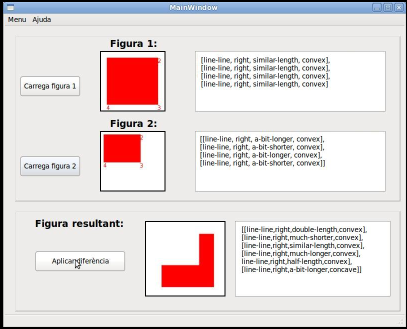
\includegraphics[width=260pt]{images/iufinal_p.png}
\caption {Interfície que mostra els resultats de la resta.}
\label {fig:iufinal}
\end{figure}

\section{Resultats obtinguts}
Per últim es mostraran diversos exemples de restes entre dos figures.
Les figures estaran acompanyades per la seua descripció qualitativa.
\\
\\

\subsection{Primer exemple}
El primer exemple consisteix en la resta d'un quadrat menys un altre quadrat.
El minuend, evidentment, serà de major tamany que el substrahend.
El resultat es pot observar en la Figura~\ref{fig:res1} i com es pot veure es descriu mitjançant un conjunt de vèrtexs de les dos figures inicials.
\\
\\

{\bf Minuend:}
\begin{figure}[!h]
\centering
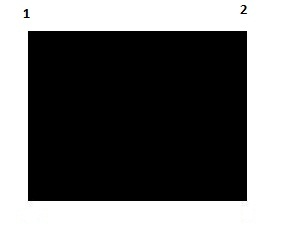
\includegraphics[width=260pt]{images/quad_gran.jpg}
\caption {Minuend del primer exemple.}
\label {fig:quad_gran1}
\end{figure}

La descripció del minuend serà:
\\
\emph {[line-line, right, similar-length, convex], [line-line, right, similar-length, convex], [line-line, right, similar-length, convex], [line-line, right, similar-length, convex]}
\\
\\

{\bf Substrahend:}
\begin{figure}[!h]
\centering
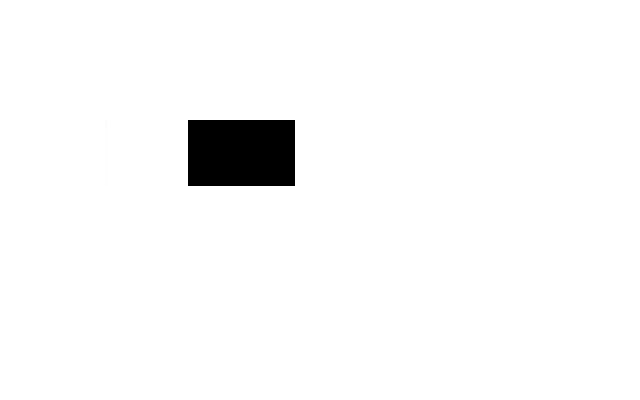
\includegraphics[width=260pt]{images/quad_menut.jpg}
\caption {Substrahend del primer exemple.}
\label {fig:quad_menut}
\end{figure}

La descripció del substrahend serà:
\\
\emph {[line-line, right, a-bit-longer, convex], [line-line, right, a-bit-shorter, convex], [line-line, right, a-bit-longer, convex], [line-line, right, a-bit-shorter, convex]}
\\
\\
{\bf Resultat:}
\begin{figure}[!h]
\centering
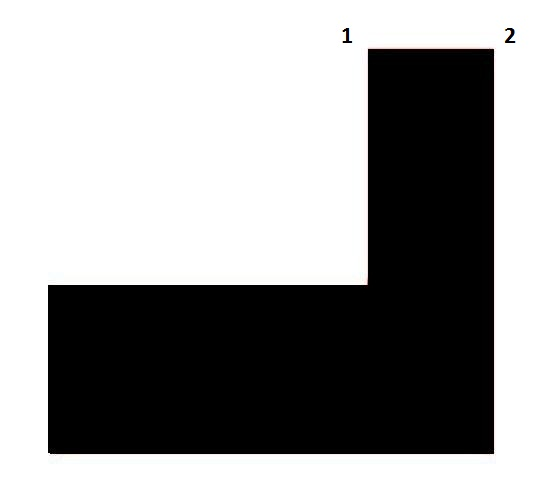
\includegraphics[width=100pt]{images/res1.jpg}
\caption {Resultat del primer exemple.}
\label {fig:res1}
\end{figure}

Finalment, la descripció de la diferència de formes quedarà:
\\
\emph {[line-line,right,double-length,convex], [line-line,right,much-shorter,convex], [line-line,right,similar-length,convex], [line-line,right,much-longer,convex], line-line,right,half-length,convex], [line-line,right,a-bit-longer,concave]}

\subsection{Segon exemple}
El segon exemple consisteix en la resta d'un quadrat menys una figura irregular en forma d'escala.
Aquest exemple mostra una major complexitat en nombre i gestió de vèrtexs-
El resultat es pot observar en la Figura~\ref{fig:res2} i descriu una figura en un nombre elevat de vèrtexs.
\\
\\

{\bf Minuend:}
\begin{figure}[!h]
\centering
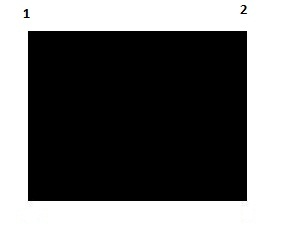
\includegraphics[width=260pt]{images/quad_gran.jpg}
\caption {Minuend del segon exemple.}
\label {fig:quad_gran2}
\end{figure}

La descripció del minuend serà:
\\
\emph {[line-line, right, similar-length, convex], [line-line, right, similar-length, convex], [line-line, right, similar-length, convex], [line-line, right, similar-length, convex]}
\\
\\

{\bf Substrahend:}
\begin{figure}[!h]
\centering

\includegraphics[width=260pt]{images/quad_escala.jpg}
\caption {Substrahend del segon exemple.}
\label {fig:quad_escala}
\end{figure}

La descripció del substrahend serà:
\\
\emph {[line-line,right,much-longer,convex], [line-line,right,a-bit-longer,convex], [line-line,obtuse,similar-length,concave], [line-line,obtuse,similar-length,convex], [line-line,obtuse,similar-length,concave], [line-line,right,similar-length,convex], [line-line,right,much-shorter,convex], [line-line,right,similar-length,convex]}
\\
\\
{\bf Resultat:}
\begin{figure}[!h]
\centering
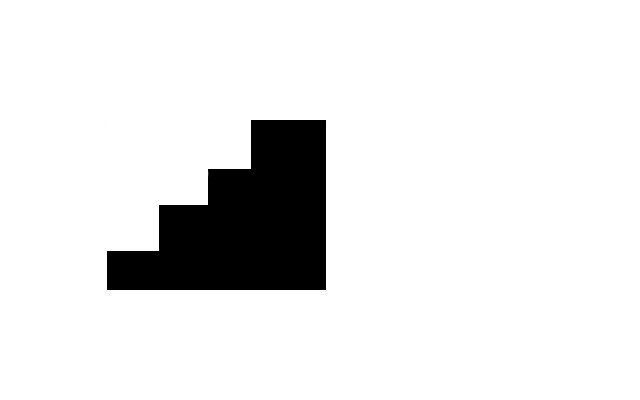
\includegraphics[width=260pt]{images/res2.jpg}
\caption {Resultat del segon exemple.}
\label {fig:res2}
\end{figure}

Finalment, la descripció de la diferència de formes quedarà:
\\
\emph {[line-line,obtuse,a-bit-longer,concave], [line-line,obtuse,a-bit-longer,convex], [line-line,obtuse,similar-length,concave], [line-line,obtuse,a-bit-shorter,convex], [line-line,obtuse,similar-length,concave], [line-line,obtuse,similar-length,convex], [line-line,obtuse,a-bit-longer,concave], [line-line,right,much-shorter,concave], [line-line,right,a-bit-longer,concave], [line-line,right,much-longer,concave]}


\subsection{Tercer exemple}
El tercer exemple consisteix en la resta d'un quadrat menys una figura que té la mateixa amplaria que el minuend.
Aquest exemple mostra un exemple dels casos en els que s'ha de descartar més d'un punt per estar repetits.
El resultat es pot observar en la Figura~\ref{fig:res3} i descriu una figura molt més estreta que l'original.
\\
\\

{\bf Minuend:}
\begin{figure}[!h]
\centering
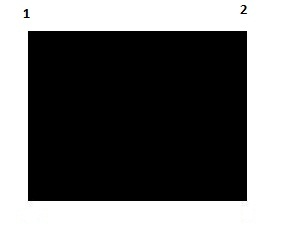
\includegraphics[width=260pt]{images/quad_gran.jpg}
\caption {Minuend del tercer exemple.}
\label {fig:quad_gran3}
\end{figure}

La descripció del minuend serà:
\\
\emph {[line-line, right, similar-length, convex], [line-line, right, similar-length, convex], [line-line, right, similar-length, convex], [line-line, right, similar-length, convex]}
\\
\\

{\bf Substrahend:}
\begin{figure}[!h]
\centering

\includegraphics[width=260pt]{images/quad_punta.jpg}
\caption {Substrahend del tercer exemple.}
\label {fig:quad_punta}
\end{figure}

La descripció del substrahend serà:
\\
\emph {[line-line,right,much-longer,convex], [line-line,right,similar-length,convex], [line-line,obtuse,a-bit-longer,concave], [line-line,right,similar-length,convex], [line-line,obtuse,a-bit-longer,convex], [line-line,obtuse,half-length,concave], [line-line,right,similar-length,convex], [line-line,right,much-shorter,convex]}
\\
\\
{\bf Resultat:}
\begin{figure}[!h]
\centering
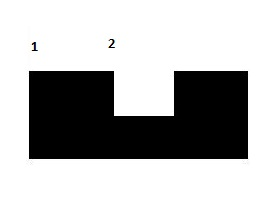
\includegraphics[width=260pt]{images/res3.jpg}
\caption {Resultat del tercer exemple.}
\label {fig:res3}
\end{figure}

Finalment, la descripció de la diferència de formes quedarà:
\\
\emph {[line-line,obtuse,similar-length,convex], [line-line,right,a-bit-longer,concave], [line-line,obtuse,a-bit-shorter,concave], [line-line,right,similar-length,convex], [line-line,right,half-length,convex], [line-line,right,a-bit-shorter,convex], [line-line,right,a-bit-longer,convex], [line-line,right,much-longer,convex]}

\subsection{Quart exemple}
El tercer exemple consisteix en la resta d'un quadrat al que ja se li ha restat una figura menys un quadrat menut.
Aquest exemple mostra un exemple de la resta sobre una figura ja modificada.
La resta s'inicia en le punt més alt i a l'esquerra del minuend.
El resultat es pot observar en la Figura~\ref{fig:res4}.
\\
\\

{\bf Minuend:}
\begin{figure}[!h]
\centering
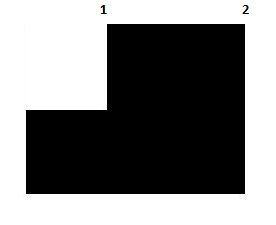
\includegraphics[width=260pt]{images/quad_gran_restat.jpg}
\caption {Minuend del quart exemple.}
\label {fig:quad_gran_restat}
\end{figure}

La descripció del minuend serà:
\\
\emph {[line-line,right,a-bit-shorter,concave], [line-line,obtuse,similar-length,convex], [line-line,right,similar-length,concave], [line-line,right,much-shorter,concave], [line-line,right,a-bit-shorter,concave], [line-line,right,a-bit-shorter,concave]}
\\
\\

{\bf Substrahend:}
\begin{figure}[!h]
\centering
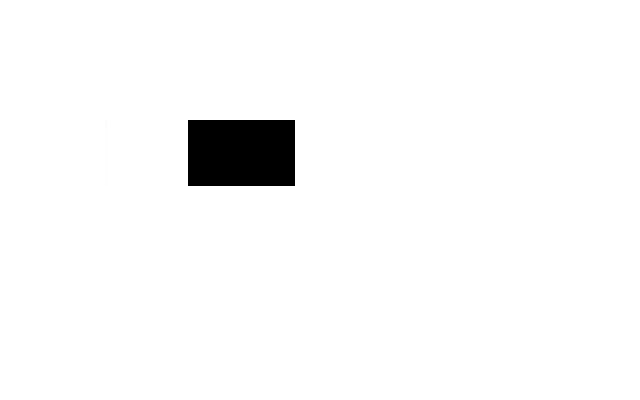
\includegraphics[width=260pt]{images/quad_menut.jpg}
\caption {Substrahend del quart exemple.}
\label {fig:quad_punta}
\end{figure}

La descripció del substrahend serà:
\\
\emph {[line-line, right, a-bit-longer, convex], [line-line, right, a-bit-shorter, convex], [line-line, right, a-bit-longer, convex], [line-line, right, a-bit-shorter, convex]}
\\
\\
{\bf Resultat:}
\begin{figure}[!h]
\centering
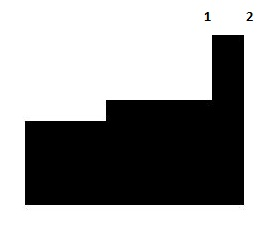
\includegraphics[width=260pt]{images/res4.jpg}
\caption {Resultat del quart exemple.}
\label {fig:res4}
\end{figure}

Finalment, la descripció de la diferència de formes quedarà:
\\
\emph {[line-line,right,much-shorter,convex], [line-line,right,a-bit-shorter,convex], [line-line,right,much-longer,convex], [line-line,right,similar-length,convex], [line-line,obtuse,much-longer,concave], [line-line,obtuse,much-shorter,convex], [line-line,obtuse,a-bit-shorter,concave], [line-line,obtuse,much-longer,convex]}
\\
\\

\section{Treball futur}
Aquest projecte es podria continuar en diverses direccions per a completar la seua aplicació.
La més important seria poder gestionar la resta quan el resultat són dos figures independents.
La informació de les dos figures no seria molt difícil de obtindre, el verdader problema resideix en la gestió de tota la imlementació per a que l'algoritme puguera ser capaç de tornar dos figures (o més) en lloc d'una única, com ara.
\\
\\
Altres millores serien la posibilitat de restar figures que no puguen ser mogudes a l'eix de coordenades.
O que aquest moviment fora opcional, per a poder restar en qualsevol zona del minuend.
\\
\\
Per últim la integració de figures en curves és un pas massa complex per a implementar-lo.
Principalment per a definir els vèrtexs de la nova figura.
 
\section{Bibliografia}
-[Mus07] L. Museros. Qualitative theory on shape representation. application to industrial manufacturing, 2007.
\\
\\
-[QR11]  L. Museros, L.González, F.Velasco i Zoe Falomir. A Qualitative Shape Description Scheme for Generating New Manufactured Shapes, Universitat Jaume I, Castellón i Universitat  Sevilla, Sevilla, Spain. 2011.
\\
\\
-[Zoe11] Zoe Falomir Llansola. Qualitative Distances and Qualitative Description of Images for Indoor Scene Description and Recognition in Robotics, Figueroles (Spain), May 13, 2011
\\
\\
-[Mus09] C4R2 No Institute Given Informe tecnico. Diferencia de formas

\end{document}

